% Options for packages loaded elsewhere
\PassOptionsToPackage{unicode}{hyperref}
\PassOptionsToPackage{hyphens}{url}
%
\documentclass[
  12pt,
]{article}
\usepackage{lmodern}
\usepackage{amssymb,amsmath}
\usepackage{ifxetex,ifluatex}
\ifnum 0\ifxetex 1\fi\ifluatex 1\fi=0 % if pdftex
  \usepackage[T1]{fontenc}
  \usepackage[utf8]{inputenc}
  \usepackage{textcomp} % provide euro and other symbols
\else % if luatex or xetex
  \usepackage{unicode-math}
  \defaultfontfeatures{Scale=MatchLowercase}
  \defaultfontfeatures[\rmfamily]{Ligatures=TeX,Scale=1}
  \setmainfont[]{Calibri Light}
\fi
% Use upquote if available, for straight quotes in verbatim environments
\IfFileExists{upquote.sty}{\usepackage{upquote}}{}
\IfFileExists{microtype.sty}{% use microtype if available
  \usepackage[]{microtype}
  \UseMicrotypeSet[protrusion]{basicmath} % disable protrusion for tt fonts
}{}
\makeatletter
\@ifundefined{KOMAClassName}{% if non-KOMA class
  \IfFileExists{parskip.sty}{%
    \usepackage{parskip}
  }{% else
    \setlength{\parindent}{0pt}
    \setlength{\parskip}{6pt plus 2pt minus 1pt}}
}{% if KOMA class
  \KOMAoptions{parskip=half}}
\makeatother
\usepackage{xcolor}
\IfFileExists{xurl.sty}{\usepackage{xurl}}{} % add URL line breaks if available
\IfFileExists{bookmark.sty}{\usepackage{bookmark}}{\usepackage{hyperref}}
\hypersetup{
  pdftitle={ Logistic Regression Modeling of the Growth Limit of Alicyclobacillus Acidoterrestris CRA7152 in Apple Juice},
  pdfauthor={Loftsson, Valentin Oliver --- valentin.loftsson@epfl.ch},
  hidelinks,
  pdfcreator={LaTeX via pandoc}}
\urlstyle{same} % disable monospaced font for URLs
\usepackage[margin=2.5cm]{geometry}
\usepackage{color}
\usepackage{fancyvrb}
\newcommand{\VerbBar}{|}
\newcommand{\VERB}{\Verb[commandchars=\\\{\}]}
\DefineVerbatimEnvironment{Highlighting}{Verbatim}{commandchars=\\\{\}}
% Add ',fontsize=\small' for more characters per line
\usepackage{framed}
\definecolor{shadecolor}{RGB}{248,248,248}
\newenvironment{Shaded}{\begin{snugshade}}{\end{snugshade}}
\newcommand{\AlertTok}[1]{\textcolor[rgb]{0.94,0.16,0.16}{#1}}
\newcommand{\AnnotationTok}[1]{\textcolor[rgb]{0.56,0.35,0.01}{\textbf{\textit{#1}}}}
\newcommand{\AttributeTok}[1]{\textcolor[rgb]{0.77,0.63,0.00}{#1}}
\newcommand{\BaseNTok}[1]{\textcolor[rgb]{0.00,0.00,0.81}{#1}}
\newcommand{\BuiltInTok}[1]{#1}
\newcommand{\CharTok}[1]{\textcolor[rgb]{0.31,0.60,0.02}{#1}}
\newcommand{\CommentTok}[1]{\textcolor[rgb]{0.56,0.35,0.01}{\textit{#1}}}
\newcommand{\CommentVarTok}[1]{\textcolor[rgb]{0.56,0.35,0.01}{\textbf{\textit{#1}}}}
\newcommand{\ConstantTok}[1]{\textcolor[rgb]{0.00,0.00,0.00}{#1}}
\newcommand{\ControlFlowTok}[1]{\textcolor[rgb]{0.13,0.29,0.53}{\textbf{#1}}}
\newcommand{\DataTypeTok}[1]{\textcolor[rgb]{0.13,0.29,0.53}{#1}}
\newcommand{\DecValTok}[1]{\textcolor[rgb]{0.00,0.00,0.81}{#1}}
\newcommand{\DocumentationTok}[1]{\textcolor[rgb]{0.56,0.35,0.01}{\textbf{\textit{#1}}}}
\newcommand{\ErrorTok}[1]{\textcolor[rgb]{0.64,0.00,0.00}{\textbf{#1}}}
\newcommand{\ExtensionTok}[1]{#1}
\newcommand{\FloatTok}[1]{\textcolor[rgb]{0.00,0.00,0.81}{#1}}
\newcommand{\FunctionTok}[1]{\textcolor[rgb]{0.00,0.00,0.00}{#1}}
\newcommand{\ImportTok}[1]{#1}
\newcommand{\InformationTok}[1]{\textcolor[rgb]{0.56,0.35,0.01}{\textbf{\textit{#1}}}}
\newcommand{\KeywordTok}[1]{\textcolor[rgb]{0.13,0.29,0.53}{\textbf{#1}}}
\newcommand{\NormalTok}[1]{#1}
\newcommand{\OperatorTok}[1]{\textcolor[rgb]{0.81,0.36,0.00}{\textbf{#1}}}
\newcommand{\OtherTok}[1]{\textcolor[rgb]{0.56,0.35,0.01}{#1}}
\newcommand{\PreprocessorTok}[1]{\textcolor[rgb]{0.56,0.35,0.01}{\textit{#1}}}
\newcommand{\RegionMarkerTok}[1]{#1}
\newcommand{\SpecialCharTok}[1]{\textcolor[rgb]{0.00,0.00,0.00}{#1}}
\newcommand{\SpecialStringTok}[1]{\textcolor[rgb]{0.31,0.60,0.02}{#1}}
\newcommand{\StringTok}[1]{\textcolor[rgb]{0.31,0.60,0.02}{#1}}
\newcommand{\VariableTok}[1]{\textcolor[rgb]{0.00,0.00,0.00}{#1}}
\newcommand{\VerbatimStringTok}[1]{\textcolor[rgb]{0.31,0.60,0.02}{#1}}
\newcommand{\WarningTok}[1]{\textcolor[rgb]{0.56,0.35,0.01}{\textbf{\textit{#1}}}}
\usepackage{graphicx,grffile}
\makeatletter
\def\maxwidth{\ifdim\Gin@nat@width>\linewidth\linewidth\else\Gin@nat@width\fi}
\def\maxheight{\ifdim\Gin@nat@height>\textheight\textheight\else\Gin@nat@height\fi}
\makeatother
% Scale images if necessary, so that they will not overflow the page
% margins by default, and it is still possible to overwrite the defaults
% using explicit options in \includegraphics[width, height, ...]{}
\setkeys{Gin}{width=\maxwidth,height=\maxheight,keepaspectratio}
% Set default figure placement to htbp
\makeatletter
\def\fps@figure{htbp}
\makeatother
\setlength{\emergencystretch}{3em} % prevent overfull lines
\providecommand{\tightlist}{%
  \setlength{\itemsep}{0pt}\setlength{\parskip}{0pt}}
\setcounter{secnumdepth}{-\maxdimen} % remove section numbering
\usepackage{fancyhdr}
\pagestyle{fancy}
\fancyhead[L]{\textit{\leftmark}}
\fancyhead[R]{Loftsson}
\usepackage{titlesec}
\titlespacing{\title}{0pt}{\parskip}{-\parskip}
\usepackage{hyperref}
\hypersetup{colorlinks=true, urlcolor=black}
\usepackage{bm}
\usepackage{amsmath}
\usepackage[font={small, color=blue}]{caption}
\usepackage{subcaption}
\usepackage{booktabs}
\usepackage{longtable}
\usepackage{array}
\usepackage{multirow}
\usepackage{wrapfig}
\usepackage{float}
\usepackage{colortbl}
\usepackage{pdflscape}
\usepackage{tabu}
\usepackage{threeparttable}
\usepackage{threeparttablex}
\usepackage[normalem]{ulem}
\usepackage{makecell}
\usepackage{xcolor}

\title{\vspace{-2cm} Logistic Regression Modeling of the Growth Limit of
Alicyclobacillus Acidoterrestris CRA7152 in Apple Juice}
\author{Loftsson, Valentin Oliver ---
\href{mailto:valentin.loftsson@epfl.ch}{\nolinkurl{valentin.loftsson@epfl.ch}}}
\date{}

\begin{document}
\maketitle

\hypertarget{introduction}{%
\section{Introduction}\label{introduction}}

Microbiological contamination in processed acid fruit juices has been
the subject of microbiological interest and research in the past few
decades. Controlling such contamination is an important factor in the
preservation of packed fruit juice products. To minimize contamination
risk, it is essential to consider changes in the microbiology of the
product over the entire production cycle, from cultivation and
harvesting to preparation, distribution, and storage.

Peña \emph{et al.} (2011) studied the contamination in apple juice
caused by an acidophilic sporeformer bacterium, \emph{Alicyclobacillus
acidoterrestris} CRA7152, and developed a model to predict its growth
probability. The bacterium causes ``off-flavor'' in fruit juices from
certain chemical compounds. Several studies have shown that
\emph{Alicyclobacillus acidoterrestris} grows at temperatures between 25
to 60°C (Previdi and Vicini 1995) with pH varying from 3.0 to 5.5
(Eguchi 1997). The use of nisin, a chemical that is used as a food
preservative, has proven effective as a minimum inhibitory concentration
method to control the germination of the bacterium's spores. However,
the effectiveness of nisin depends also on the temperature, pH, and
soluble solids concentration.

Evaluating the bacterium's growth/nongrowth interface becomes cumbersome
when multiple factors are involved. Logistic regression is a powerful
tool for probabilistic microbial modeling, given that sufficient
information is available about the product characteristics and
conditions. It has been used frequently in similar studies. With
logistic regression, it is possible to describe the growth probability
and establish critical limits for the predictive variables that describe
the condition of the apple juice.

In this paper, we reproduce the statistical analyses performed by Peña
\emph{et al.} on the original dataset. One main purpose of the original
study is to ``evaluate the growth responses of \emph{Alicyclobacillus
acidoterrestris} in apple juice with different pH values, concentrations
of soluble solids and nisin subjected to different incubation
temperatures''. We begin with an exploratory data analysis and then
perform a logistic regression analysis to determine and evaluate an
optimal predictive model.

\hypertarget{exploratory-data-analysis}{%
\section{Exploratory Data Analysis}\label{exploratory-data-analysis}}

The dataset includes 74 samples of apple juice assays including a binary
growth response (0=No Growth, 1=Growth) evaluated after 16 days of
incubation. The dataset consists of two collections of 37 assays, tested
in duplicate. The assays were carefully created by the researchers to
ensure a balanced dataset with a varied combination of factors to
determine the juice condition.

The effect of four factors was studied as summarized in
\hyperref[table1:ph]{Tables 1-4}. The frequency table of the growth
response reveals that we have a semi-balanced dataset, with several more
negative examples and growth occurring in 26 out of 74 assays (\(\sim\)
35\%). Here, the response is categorical and the covariate values are
discrete, so it is natural to use frequency tables. For each factor,
four discrete values were selected for testing after careful
experimentation and analysis, and considering accumulated knowledge from
previous studies. The tables reveal some interesting characteristics
about individual factors independent of interaction effects: Growth was
completely inhibited at pH 3.5 (\hyperref[table1:ph]{Table 1}) which is
the minimum pH of the juice. It was also fully inhibited at the maximum
nisin concentration 70 IU/ml (\hyperref[table2:nisin]{Table 2}) and at
the maximum soluble solids concentration of 19 °Brix
(\hyperref[table4:brix]{Table 4}), which marks the concentration level
above which no growth of \emph{A. acidoterrestris} occurs
(Splittstoesser, Churey, and Lee 1994).

\begin{figure}
\centering
\begin{minipage}{.5\textwidth}
  \centering
  \caption*{}
  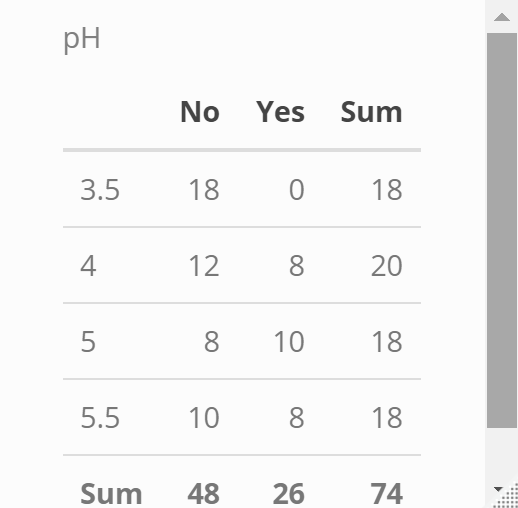
\includegraphics[width=\linewidth]{ph}
  \label{table1:ph}
\end{minipage}%
\begin{minipage}{.5\textwidth}
  \centering
  \caption*{}
  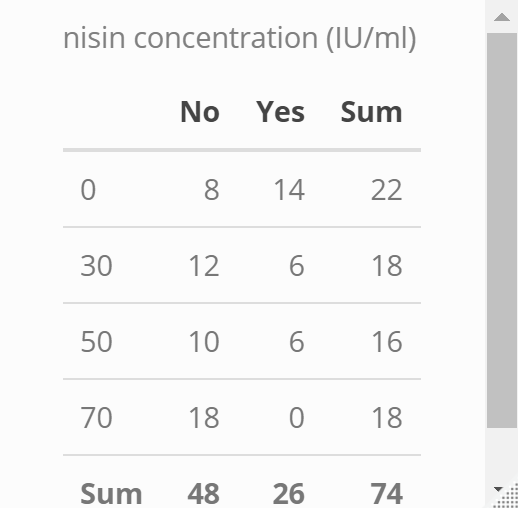
\includegraphics[width=\linewidth]{nisin}
  \label{table2:nisin}
\end{minipage}
\end{figure}

\begin{figure}
\centering
\begin{minipage}{.5\textwidth}
  \centering
  \caption*{}
  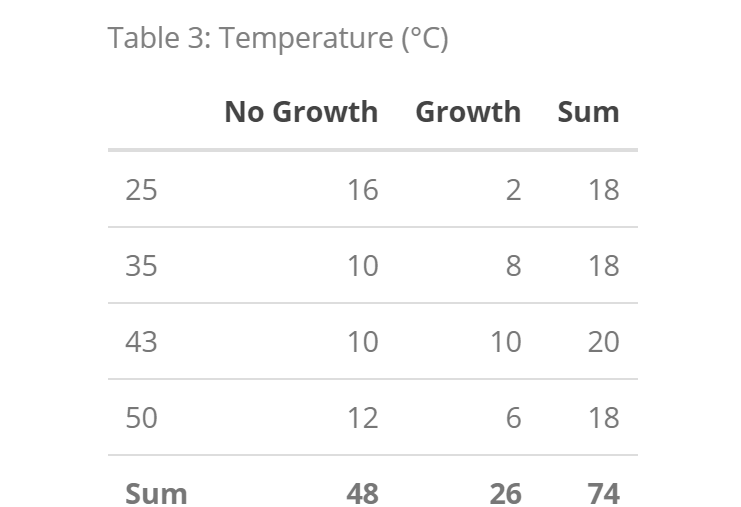
\includegraphics[width=\linewidth]{temperature}
  \label{table3:temperature}
\end{minipage}%
\begin{minipage}{.5\textwidth}
  \centering
  \caption*{}
  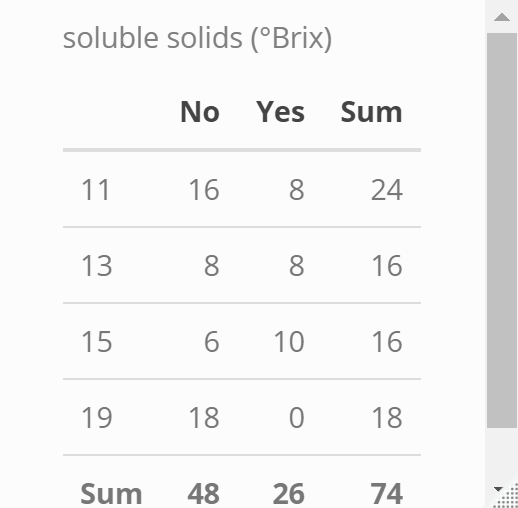
\includegraphics[width=\linewidth]{brix}
  \label{table4:brix}
\end{minipage}
\end{figure}

\hypertarget{model-fitting-and-selection}{%
\section{Model Fitting and
Selection}\label{model-fitting-and-selection}}

Logistic regression is used as a method for model fitting as it is
suitable for a binary response. Here, we use the logit function as the
link transformation for the generalized model:

\begin{equation}
logit(p) = log(\frac{p}{1-p}) = \beta_0 + \beta_1x_1 + \beta_2x_2 + \dots + \beta_kx_k
\end{equation}

Essentially, this means that the linear transformation outputs the logit
transformed probability of a positive response (\(Y=Growth\)). To obtain
the probability, \(p\), we must apply the inverse logit function:

\begin{equation}
p = \frac{\exp(\beta_0 + \beta_1x_1 + \beta_2x_2 + \dots + \beta_kx_k)}{1 + \exp(\beta_0 + \beta_1x_1 + \beta_2x_2 + \dots + \beta_kx_k)}
\end{equation}

The parameters \(\beta_k\) are estimated by maximum likelihood.

To capture important characteristics of relationships between the
explanatory variables, we start with a model that includes all main and
interaction effects. Note that \texttt{\^{}2} denotes the inclusion of
all interaction effects:

\begin{Shaded}
\begin{Highlighting}[]
\NormalTok{growth }\OperatorTok{~}\StringTok{ }\NormalTok{(ph }\OperatorTok{+}\StringTok{ }\NormalTok{nisin }\OperatorTok{+}\StringTok{ }\NormalTok{temperature }\OperatorTok{+}\StringTok{ }\NormalTok{brix)}\OperatorTok{^}\DecValTok{2}
\end{Highlighting}
\end{Shaded}

A likelihood-ratio test (LRT) was used to perform backward variable
selection. The LRT compares two models where one is a sub-model of the
other, by computing the LR test statistic, denoted here as \(\lambda\):

\begin{equation}
\lambda = -2\ln{\frac{L(m_1)}{L(m_2)}} = 2(\ln{L(m_2)} - \ln{L(m_1)})
\end{equation}

where \(m_1\) corresponds to the more restrictive model and \(m_2\) is
the less restrictive model. \(L(*)\) denotes the likelihood of the data
samples given a model. The statistic is Chi-squared distributed.

The LRT essentially tests the following null and alternative hypotheses:

\begin{itemize}
\tightlist
\item
  \textbf{H}: \(\beta_k = 0\) for all variables \(k\) that differ
  between the models
\item
  \textbf{A}: \(\beta_k \neq 0\)
\end{itemize}

\begin{figure}
\centering
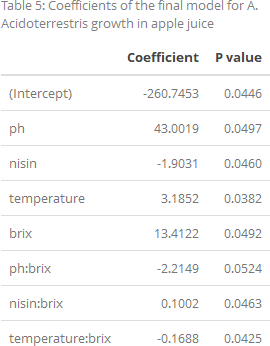
\includegraphics{table5}
\caption*{}
\label{table5}
\end{figure}

For each factor, we compare the full model described above against the
sub-model with that factor removed. The results can be viewed in
\hyperref[table5]{Table 5}. Clearly, the terms \texttt{ph:nisin},
\texttt{ph:temperature}, and \texttt{nisin:temperature} are not
significant as their P-values indicate (P \textgreater{} 0.05). As a
result, we do not reject the null hypothesis that the coefficients for
these terms are zero and they are thus dropped from the model.

\hypertarget{final-model}{%
\section{Final Model}\label{final-model}}

The remaining terms of the final model are all the main effects and
interactions of \texttt{brix} with each variable. The coefficients and
corresponding P-values are presented in \hyperref[table6]{Table 6}.
Below is the model in mathematical terms: \begin{multline}
logit(p(Growth)) = -260.7453 \\
+ 43.0019\cdot\pmb{pH} - 1.9031\cdot\pmb{nisin} + 3.1852\cdot\pmb{temp} + 13.4122\cdot\pmb{brix} \\
- 2.2149\cdot\pmb{pH}\cdot\pmb{brix} + 0.1002\cdot\pmb{nisin}\cdot\pmb{brix} - 0.1688\cdot\pmb{temp}\cdot\pmb{brix}
\end{multline}

\(~\)

\begin{figure}
\centering
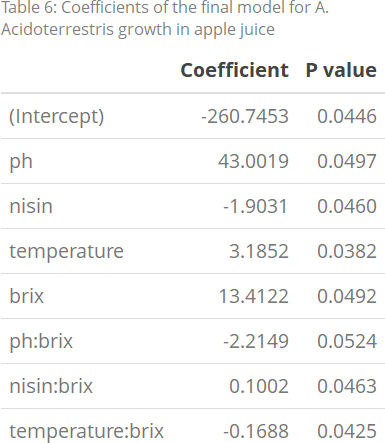
\includegraphics{table6}
\caption*{}
\label{table6}
\end{figure}

\hypertarget{model-evaluation}{%
\section{Model Evaluation}\label{model-evaluation}}

The model concordance or classification accuracy was used to assess the
model's performance. The resulting confusion matrix is presented in
\hyperref[table7]{Table 7}. The overall accuracy is 97.3\%, meaning only
2.7\% or 2 samples out of 74 were incorrectly classified. The final
model and accuracy results match the findings of Peña \emph{et al.}
(2011).

\begin{figure}
\centering
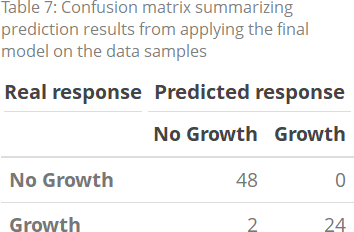
\includegraphics{table7}
\caption*{}
\label{table7}
\end{figure}

Peña \emph{et al.} (2011) confirmed the validity of the model through
experiments on new samples. These experiments testified to the
usefulness of nisin in preventing the growth of the bacterium and
thereby increasing the shelf life of apple juice, especially under
conditions of high temperature.

We visualize the behavior of the final model on surface graphs
(\hyperref[fig1a]{Figures 1-2}). The graphs show the predicted growth
probability of \emph{A. acidoterrestris} in apple juice as a function of
two main effects. The graphs can be explored interactively online by
clicking the links above the figure captions.

\hyperref[fig1a]{Figures 1.a and 1.b} show the probability as a function
of soluble solids concentration and temperature, given 0 IU/ml of nisin
and pH 3.7 and 4.5, respectively. For pH 4.5
(\hyperref[fig1b]{Figure 1.b}), growth was inhibited only in high
concentrations of soluble solids (Brix). Interestingly, when pH drops
down to 3.7 (\hyperref[fig1a]{Figure 1.a}) no growth occurs for any
value of Brix up to a temperature of 30°C. Above 30°C, the probability
is close to zero only above 18°Brix.

\hyperref[fig2a]{Figures 2.a and 2.b} show the probability as a function
of soluble solids concentration and nisin concentration, given pH 4.0
and temperature 45°C and 30°C, respectively. For 45°C
(\hyperref[fig2a]{Figure 2.a}) growth can be inhibited by adding 40-70
IU/ml of nisin. When the temperature is decreased to 30°C
(\hyperref[fig2b]{Figure 2.b}) we observe that the model predicts zero
or small probability of growth for any Brix level and low nisin levels.
At zero nisin, the probability grows smaller as Brix the level grows
higher.

The graphs show the effect and interactions of the variables and reveal
critical values that are important to establish minimum inhibitory
limits. Such limits are necessary for minimizing the use of inhibitory
chemicals in the product and depend on the pH and temperature levels.
Peña \emph{et al.} discuss critical boundaries in more detail.

\begin{figure}
\centering
\begin{minipage}{.5\textwidth}
  \centering
  \caption*{\hypersetup{urlcolor=blue}\href{https://chart-studio.plotly.com/~valentinoli/7/}{View interactive plot online}}
  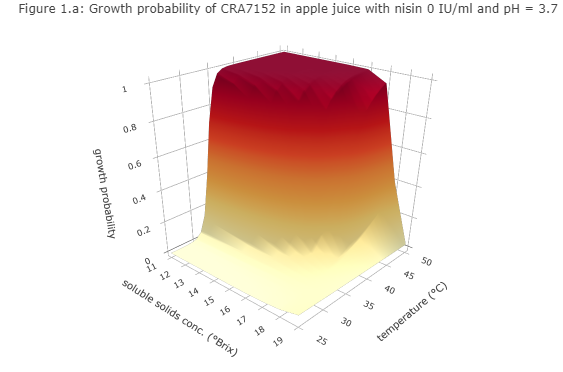
\includegraphics[width=\linewidth]{fig1a}
  \label{fig1a}
\end{minipage}%
\begin{minipage}{.5\textwidth}
  \centering
  \caption*{\hypersetup{urlcolor=blue}\href{https://chart-studio.plotly.com/~valentinoli/9/}{View interactive plot online}}
  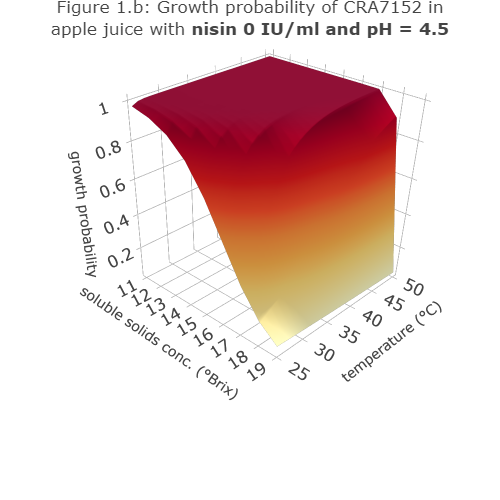
\includegraphics[width=\linewidth]{fig1b}
  \label{fig1b}
\end{minipage}
\end{figure}

\begin{figure}
\centering
\begin{minipage}{.5\textwidth}
  \centering
  \caption*{\hypersetup{urlcolor=blue}\href{https://chart-studio.plotly.com/~valentinoli/11/}{View interactive plot online}}
  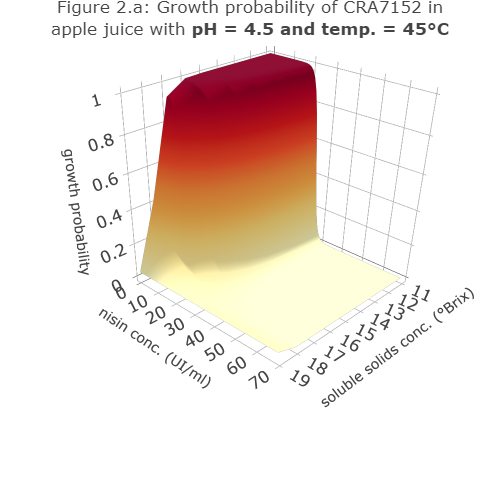
\includegraphics[width=\linewidth]{fig2a}
  \label{fig2a}
\end{minipage}%
\begin{minipage}{.5\textwidth}
  \centering
  \caption*{\hypersetup{urlcolor=blue}\href{https://chart-studio.plotly.com/~valentinoli/13/}{View interactive plot online}}
  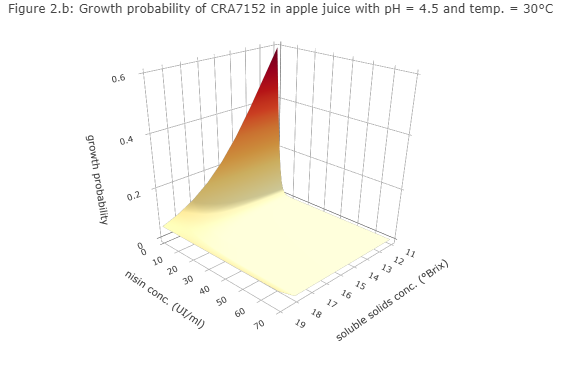
\includegraphics[width=\linewidth]{fig2b}
  \label{fig2b}
\end{minipage}
\end{figure}

\hypertarget{conclusion}{%
\section{Conclusion}\label{conclusion}}

In this paper, we set out to reproduce the work of Peña \emph{et al.}
(2011) to develop a model to predict growth probabilities of
\emph{Alicyclobacillus acidoterrestris} in apple juice depending on pH,
incubation temperature, soluble solids, and nisin concentration. We
successfully fit the data using logistic regression and found an optimal
model using stepwise model selection. The results match the findings of
the original study. Since the final model includes both main and
interaction terms, the model coefficients are not easily interpretable.
Nevertheless, the model's prediction accuracy has been verified through
accuracy testing, visualization, and experimentation. The model provides
a beneficial tool for apple juice production since it can be used to
minimize the risk of bacterial spoilage in apple juice.

\hypertarget{software}{%
\section{Software}\label{software}}

The reproduction was performed in the \texttt{R} programming language (R
Core Team 2019). Tables were created with \texttt{kableExtra} (Zhu
2019). Interactive figures were created with Plotly (Sievert 2020).

\hypertarget{references}{%
\section*{References}\label{references}}
\addcontentsline{toc}{section}{References}

\hypertarget{refs}{}
\leavevmode\hypertarget{ref-eguchi}{}%
Eguchi, S. Y. et al. 1997. ``Detection of Acidothermophilic Bacilli in
Industrialized Fruit Juices, Fruit Processing.'' \emph{FRUIT
PROCESSING}, FRUIT processing, 7 (9): 350--53.
\url{https://www.tib.eu/de/suchen/id/BLSE\%3ARN032043094}.

\leavevmode\hypertarget{ref-pena}{}%
Peña, Wilmer, Pilar Massaguer, A. D.G. ZUÑIGA, and Sergio Saraiva. 2011.
``Modeling the Growth Limit of Alicyclobacillus Acidoterrestris Cra7152
in Apple Juice: Effect of pH, Brix, Temperature and Nisin
Concentration.'' \emph{Journal of Food Processing and Preservation} 35
(August). \url{https://doi.org/10.1111/j.1745-4549.2010.00496.x}.

\leavevmode\hypertarget{ref-previdi}{}%
Previdi, Colla, M. P., and E. Vicini. 1995. ``Characterization of
Alicyclobacillus, a Spore-Forming Thermophilic Acidophilic Bacterium.''
\emph{The Indian Journal of Soil Conservation}, no. 70: 128--32.

\leavevmode\hypertarget{ref-r}{}%
R Core Team. 2019. \emph{R: A Language and Environment for Statistical
Computing}. Vienna, Austria: R Foundation for Statistical Computing.
\url{https://www.R-project.org/}.

\leavevmode\hypertarget{ref-plotly}{}%
Sievert, Carson. 2020. \emph{Interactive Web-Based Data Visualization
with R, Plotly, and Shiny}. Chapman; Hall/CRC.
\url{https://plotly-r.com}.

\leavevmode\hypertarget{ref-splittstoesser}{}%
Splittstoesser, DF, JJ Churey, and CY Lee. 1994. ``Growth
Characteristics of Aciduric Sporeforming Bacilli Isolated from Fruit
Juices.'' \emph{Journal of Food Protection} 57 (12): 1080---1083.
\url{https://doi.org/10.4315/0362-028x-57.12.1080}.

\leavevmode\hypertarget{ref-kableExtra}{}%
Zhu, Hao. 2019. \emph{KableExtra: Construct Complex Table with 'Kable'
and Pipe Syntax}. \url{https://CRAN.R-project.org/package=kableExtra}.

\end{document}
